\documentclass{paper}
\usepackage{sbc-template}

\usepackage{proof}
\usepackage{mathpartir}
\usepackage{amsmath}
\usepackage{amssymb}
\usepackage{graphicx}
\usepackage{listings}
\usepackage{float}

\newtheorem{theorem}{Theorem}[section]
\newtheorem{corollary}[theorem]{Corollary}
\newtheorem{lemma}[theorem]{Lemma}
\newtheorem{definition}[theorem]{Definition}

\def\qed{\unskip\kern 10pt{\unitlength1pt\linethickness{.4pt}\framebox(6,6){}}}

\newcommand{\fun}[1]{\mbox{\textbf{#1}}}
\newcommand{\lb}[1]{#1_{\downarrow}}
\newcommand{\ub}[1]{#1_{\uparrow}}
\newcommand{\varset}[1]{\mbox{$\cal{#1}$}}

\sloppy


\begin{document}
\lstset{language=, basicstyle=\small} 

\title{A Tool for Range Analysis of Whole Programs}

\author{Victor Hugo Sperle Campos, Raphael Ernani Rodrigues, \\
Igor Rafael de Assis Costa, Douglas do Couto Teixeira \\
and Fernando Magno Quint\~{a}o Pereira}

\address{UFMG -- 6627 Ant\^{o}nio Carlos Av, 31.270-010, Belo Horizonte, Brazil
\email{\{victorsc,raphael,igor,douglas,fernando\}@dcc.ufmg.br}
}


\maketitle

%mmmmmmmmmmmmmmmmmmmmmmmmmmmmmmmmmmmmmmmmmmmmmmmmmmmmmmmmmmmmmmmmmmmmmmmmmmmmmm
\begin{abstract}
Range analysis is a compiler technique that determines statically the lower and
upper values that each integer variable from a target program may assume
during this program's execution.
This type of inference is very important, because it enables several compiler
optimizations, such as dead and redundant code elimination, bitwidth aware
register allocation, and detection of program vulnerabilities.
In this paper we present a tool that implements an inter-procedural,
context-sensitive  range analysis algorithm for the LLVM compiler.
Our tool can be used as a standalone compiler pass that gives the user
static information about the variables in a program, or it can be used to
enable other compiler optimizations.
This tool has been implemented to be able to scale to large code bodies.
As an example, we have used it to analyze the whole gcc compiler is less than
15 seconds.
\end{abstract}

\section{Introduction}
\label{sec:intro}

% The context: why range analysis is necessary.
The analysis of integer variables on the interval lattice has been the
canonical example of abstract interpretation since its introduction in
Cousot and Cousot's seminal paper~\cite{Cousot77}.
Compilers use range analysis to infer the possible values that discrete
variables may assume during program execution.
This analysis has many uses.
For instance, it allows the optimizing compiler to remove from the program text
redundant overflow tests~\cite{Sol11} and unnecessary array bound
checks~\cite{Bodik00}.
Additionally, range analysis is essential not only to the bitwidth aware
register allocator~\cite{Barik06}, but also to more traditional
allocators that handle registers of different
sizes~\cite{Pereira08}.
Finally, range analysis has also seen use in the static prediction of
branches~\cite{Patterson95}, to detect buffer overflow
vulnerabilities~\cite{Simon08}, to find the trip count of
loops~\cite{Lokuciejewski09}
and even in the synthesis of hardware~\cite{Mahlke01}.

% Tool capabilities.
We have implemented a range analysis tool on top of the LLVM
compiler~\cite{Lattner04}.
This tool can be used either as a standalone analysis, or it can be called by a
client pass in order to feed this client with more information about the
program.
One of our main concerns when developing our range analysis was scalability,
and we believe that our final product meets the requirements of
industrial-quality software.
We have used it to analyze a test suite with 2.72 million lines of C code.
Our implementation is fast: it globally analyzes the gcc source code in less than
15 seconds, for instance. 
It is also precise: our results are similar to Stephenson
{\em et al}'s~\cite{Stephenson00}, even though our analysis does not require
a backward propagation phase.
Furthermore, we have been able to find tight bounds to the majority of the
examples used by Costan {\em et al.}~\cite{Costan05} and Lakhdar
{\em et al.}~\cite{Lakhdar11}, who rely on much more costly methods.
In Section~\ref{sec:dsc} we provide a description of our implementation.

% The demo tool.
\noindent
\textbf{Software: }
Our tool is publicly available for
download at \texttt{http://code.google.com/p/range-analysis/}.
In our webpage we provide, in addition to the static range analysis itself,
a profiler that records the minimum and maximum values assigned to each
variable during program execution.
We also provide a visual interval to our tool, which lets the user to
see the control flow graph of the target program.
This visual interface also lets the user to see the integer intervals that
the analysis estimates to each variable.

% The rest of this paper.

\section{Algorithm Description}
\label{sec:dsc}

% Define the lattice, the constraints and the valuation I.
\noindent
\textbf{The Interval Lattice.}
We perform arithmetic operations over the complete lattice
$\cal{Z} = \mathbb{Z} \cup \{-\infty, +\infty\}$, where the ordering is
naturally given by $-\infty < \ldots < -2 < -1 < 0 < 1 < 2 < \ldots +\infty$.
For any $x > -\infty$ we define:

\begin{tabular}{lcl}
$x + \infty = \infty, x \neq -\infty$ & \mbox{\hspace{0.1cm}} & $x - \infty = - \infty, x \neq +\infty$ \\
$x \times \infty = \infty$ if $x > 0$ & & $x \times \infty = -\infty$ if $x < 0$ \\
$0 \times \infty = 0$ & & $(-\infty) \times \infty = \ $ not defined  \\
\end{tabular}

From the lattice $\varset{Z}$ we define the product lattice
$\varset{Z}^2$, which is partially ordered by the subset relation
$\sqsubseteq$.
$\varset{Z}^2$ is defined as follows:
%
\begin{equation*}
\varset{Z}^2 = \emptyset \cup \{[z_1, z_2] | \ z_1,z_2 \in \varset{Z},
\ z_1 \leq z_2, \  -\infty < z_2 \}
\end{equation*}
%
The objective of range analysis is to determine a mapping
$I: \varset{V} \mapsto \varset{Z}^2$ from the set of integer program variables
$V$ to intervals, such that, for any variable $v \in V$, if
$I(v) = [l, u]$, then, during the execution of the target program, any
value $i$ assigned to $v$ is such that $l \leq i \leq u$.

\noindent
\textbf{A Holistic View of our Range Analysis Algorithm.}
We perform range analysis in a number of steps.
First, we convert the program to a suitable intermediate representation that
makes it easier to extract constraints.
From these constraints, we build a dependence graph that allows us to do
range analysis sparsely.
Finally, we solve the constraints applying different fix-point iterators on
this dependence graph.
Figure~\ref{fig:algorithm} gives a global view of this algorithm.
Some of the steps in the algorithm are optional.
They improve the precision of the range analysis, at the expense of a longer
running time.
The last phase happens per strong component; however, if we opted for not building 
these components, then it happens once for the entire constraint graph.
Nevertheless, the use of strongly connected components
is so essential for performance and precision that it is considered optional only because we
can easily build our implementation without this module.


\begin{figure}[h]
\begin{center}
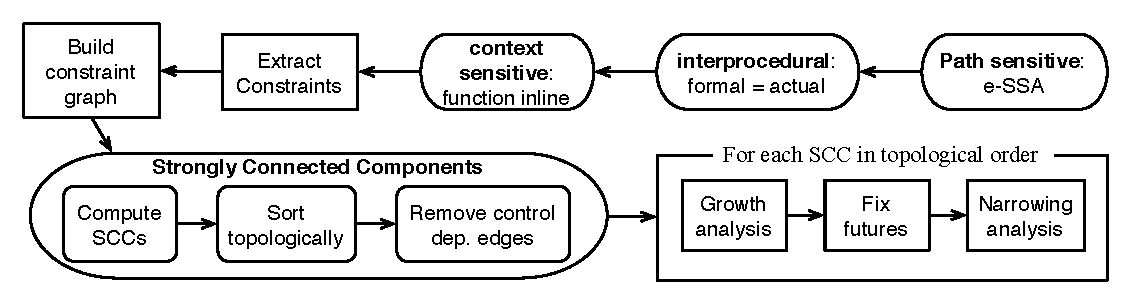
\includegraphics[width=\textwidth]{images/algorithm}
\end{center}
\caption{\label{fig:algorithm}
Our implementation of range analysis. Rounded boxes are optional steps.}
\end{figure}

\begin{figure}[H]
\begin{center}
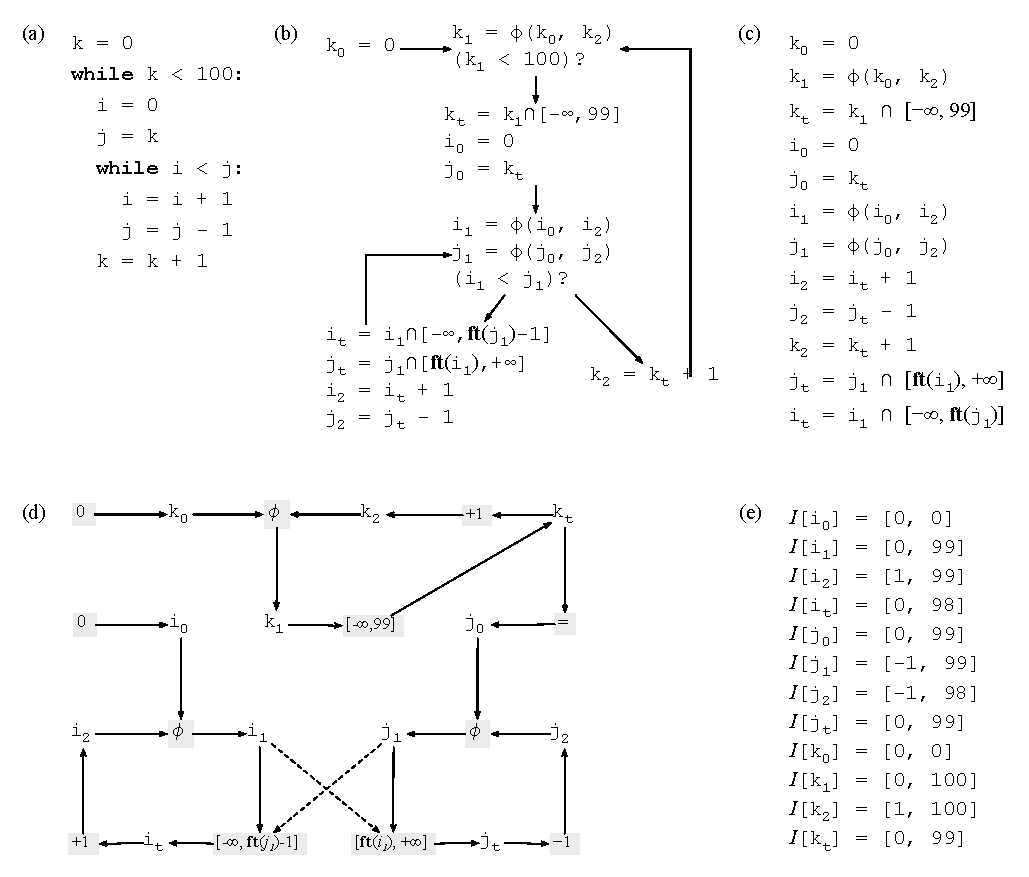
\includegraphics[width=\textwidth]{images/overall_view}
\end{center}
\caption{\label{fig:overall_view}
Range analysis by example.
(a) Input program.
(b) Internal compiler representation.
(c) Constraints of the range analysis problem.
(d) The constraint graph.
(e) The final solution.}
\end{figure}

We will illustrate the mandatory parts of the
algorithm via the example program in Figure~\ref{fig:overall_view}.
Figure~\ref{fig:overall_view}(a) shows a program taken from the
partition function of the quicksort algorithm used by Bodik
{\em et al.}~\cite{Bodik00}.
We have removed the code that performs array manipulation from this program,
as it plays no role in our explanation.
Figure~\ref{fig:overall_view}(b) shows one possible way to represent this
program internally.
A good program representation allows us to find more precise results.
In this example we chose a program representation called
Extended Static Single Assignment form~\cite{Bodik00}, which lets us to solve
range analysis via a path sensitive algorithm.
Figure~\ref{fig:overall_view}(c) shows the constraints that we extract from
the intermediate representation seen in part (b) of this figure.
From these constraints we build the {\em constraint graph} in
Figure~\ref{fig:overall_view}(d).
This graph is the main data-structure that we use to solve range analysis.
For each variable $v$ in the constraint system, the constraint graph has a node
$n_v$.
Similarly, for each operation $v = f(\ldots, u, \ldots)$ in the program, the
graph has an {\em operation node} $n_f$.
For each operation $v = f(\ldots, u, \ldots)$ we add two edges to the
graph: $\overrightarrow{n_un_f}$ and $\overrightarrow{n_fn_v}$.
Some edges in the constraint graph are dashed.
These are called {\em control dependence edges}.
If a constraint $v = f(\ldots, \fun{ft}(u), \ldots)$ uses a {\em future}
bound from a variable $u$, then we add to the constraint graph a control
dependence edge $\overrightarrow{n_un_f}$.
Futures are symbolic expressions, which denote intervals whose limits are
not known immediately, but might be known after the analysis starts solving
the constraints.
The final solution to this instance of the range analysis problem is
given in Figure~\ref{fig:overall_view}(e).



\section{How to Create a LLVM pass using our Analysis}
\label{sec:howto}

Our analysis can be used independently from other compiler clients, to identify
logical problems in the analyzed code.
However, the Range Analysis is more often used as a tool to identify dead code,
memory overflow and redundant checks; hence, enabling other compiler analysis.
We will illustrate this last mode via an example.
In order to use our range analysis, one can write a LLVM pass that calls it.
There is vast documentation~\footnote{\texttt{http://llvm.org/docs/WritingAnLLVMPass.html}} about how to write LLVM passes in the web.
The program below, which is self-contained, is an example of such a pass.
This program is a LLVM pass; that is, it is called as part of the LLVM
tool chain, and receives as input a data-structure of the \texttt{Function}
type, that describes the program.
An iterator over such a data-structure returns a list of basic blocks.
Iterators over basic-blocks return a list of instructions.

%Example pass: Source code
\begin{lstlisting}[frame=single]
//We are ommiting the LLVM includes
#include "../RangeAnalysis/RangeAnalysis.h"
using namespace llvm;
class ClientRA: public llvm::FunctionPass {
public:
  static char ID;
  ClientRA() : FunctionPass(ID){ }
  virtual ~ClientRA() { }
  virtual bool runOnFunction(Function &F){
    IntraProceduralRA<Cousot> &ra = getAnalysis<IntraProceduralRA<Cousot>>();
    errs() << "\nCousot Intra Procedural analysis 
               (Values -> Ranges) of " << F.getName() << ":\n";
    for(Function::iterator bb=F.begin(), bbEnd=F.end(); bb!=bbEnd; ++bb){
      for(BasicBlock::iterator I=bb->begin(), IEnd=bb->end(); I!=IEnd; ++I){
        if(I->getOpcode() == Instruction::Store){
          const Value *v = &(*I);
          Range r = ra.getRange(v);
          r.print(errs());
          I->dump();
        }
      }
    }
    return false;
  }

  virtual void getAnalysisUsage(AnalysisUsage &AU) const {
    AU.setPreservesAll();
    AU.addRequired<IntraProceduralRA<Cousot> >();
  }
};

char ClientRA::ID = 0;
static RegisterPass<ClientRA> 
	X("client-ra", "A client that uses RangeAnalysis", false, false);
\end{lstlisting}

Our Range Analysis interface provides a method, \textit{getRange}, that returns
a \textit{Range} object for any variable in the original code.
This object, of type \textit{Range}, contains the range information related to
the variable.
There are many versions of our range analysis pass, e.g., intra/inter procedural,
with different narrowing operators, etc.
In this example we are using the intra-procedural version using
Cousot \& Cousot's original narrowing operator~\cite{Cousot77}.

%Steps to compile and run
In order to use the example client, you need to give it a bitcode input file. Below we show how to do this.
First, we can translate a c file into a bitcode file using clang:
\begin{lstlisting}[frame=single]
clang -c -emit-llvm test.c -o test.bc
\end{lstlisting}
Next thing: we must convert the bitcode file to e-SSA form.
We do it using the \textit{vssa} pass.
The e-SSA conversion module is distributed together with our analysis; however,
its use is not mandatory.
It increases the precision of the analysis, at the expenses of a small slowdown.
In our experiments, we have observed that this slowdown is very small.
\begin{lstlisting}[frame=single]
opt -instnamer -mem2reg -break-crit-edges test.bc -o test.bc
opt -load LLVM_SRC_PATH/Debug/lib/vSSA.so -vssa test.bc -o test.essa.bc
\end{lstlisting}

Notice that we use a number of other passes too, to improve the quality of the
code that we are producing:
\textit{instnamer} just assigns strings to each variable.
We only use this pass for aesthetic reasons.
This pass will help our visual interface to look nicer.
\textit{mem2reg} maps variables allocated in the stack to virtual registers.
Without this pass everything is mapped into memory, and then our range analysis
will not be able to find any meaningful ranges to the variables.
\textit{break-crit-edges} removes the critical edges from the control flow graph
of the input program.
This pass will increase the precision of our range analysis (just a tiny bit
though), because the e-SSA transformation will be able to convert more variables
into a better format.
We run the example client with the commands below:
\begin{lstlisting}[frame=single]
opt -load LLVM_SRC_PATH/Debug/lib/RangeAnalysis.so 
    -load LLVM_SRC_PATH/Debug/lib/ClientRA.so -client-ra test.essa.bc
\end{lstlisting}
This sequence of calls will cause our example pass to be dynamically loaded
by the LLVM framework.
It will receive the bitcodes that we had produced before, and will produce,
as output, a list of variables, followed by their intervals.



\bibliographystyle{plain}
\bibliography{../references}

\end{document}
